%% Causal Claim-to-Trust Graph -- AAAI-format workshop paper
%% Toggle anonymous review version: uncomment the next line (or compile with -jobname / \def on the command line)
\def\aaaianonymous{true}
\documentclass[letterpaper]{article}
\ifdefined\aaaianonymous
  \usepackage[submission]{aaai2026}
\else
  \usepackage{aaai2026}
\fi
\usepackage{times}
\usepackage{helvet}
\usepackage{courier}
\usepackage[hyphens]{url}
\usepackage{graphicx}
\urlstyle{rm}
\def\UrlFont{\rm}
\usepackage{natbib}
\usepackage{caption}
\frenchspacing
\setlength{\pdfpagewidth}{8.5in}
\setlength{\pdfpageheight}{11in}
\usepackage{booktabs}
\usepackage{amsmath}
\usepackage{tikz}
\usetikzlibrary{arrows.meta,positioning,fit}
\pdfinfo{/TemplateVersion (2026.1)}
\setcounter{secnumdepth}{2}

\newcommand{\dT}{\Delta T}
\newcommand{\dTs}{\Delta T^{*}}

\title{Causal Claim-to-Trust Graph: Calibrating Long-Horizon Trust\\from Claim-Level Failure Provenance}
\author{Anonymous Submission}
\affiliations{}

\begin{document}
\maketitle

\begin{abstract}
Long-running LLM agent systems reuse the same specialized subagents again and again, so a supervisor's trust in each of them is state that carries forward. Yet when a recommendation is rejected, the supervisor usually learns only that the agent was wrong. The same wrong answer can come from missing context, a failed tool, a task routed to the wrong specialist, or a genuine reasoning weakness, and each cause implies a different future. We propose a Causal Claim-to-Trust Graph that extends claim-level provenance with failure cause, persistence, scope and resolution state, and we build CausalTrustBench, a matched counterfactual benchmark (200 base tasks, 800 episodes) in which the subagent, task, wrong recommendation and rejection are held fixed and only the cause changes. Across three model families and one heterogeneous team, supervisors with outcome-only memory over-penalize resolved transient failures and under-react to persistent weakness. Cause-aware graph state lowers delegation regret and false-claim survival, and a scoped update rule driven by the true cause removes most of the calibration error (trust-calibration error $0.068\to0.024$). But the graph by itself does not consistently beat a skill-conditioned baseline, and a rule driven by LLM-inferred causes recovers only part of the gain, mainly because supervisors rarely recognize missing context. Downstream task success barely moves, so the benefit lies in oversight decisions rather than accuracy.
\end{abstract}

\section{Introduction}
Imagine a lead agent that hands a multi-hop question to a specialist, receives a confident wrong answer, and rejects it. What should the lead agent believe about that specialist tomorrow? If the retrieval tool timed out, the specialist did nothing wrong and deserves the same trust as before. If the question was simply outside its remit, the right move is to route that kind of question elsewhere, while still using the specialist for its own work. If it had every fact it needed and still got the answer wrong, the weakness is real and probably will recur. Three different futures follow from one observable event.

Most memory designs for agent systems do not distinguish these cases. They record that the agent failed, perhaps against a skill label, and let later decisions inherit the penalty. In long-horizon settings this is costly in both directions: a capable specialist gets sidelined after a tool outage, and a weak one stays in the loop because a single failure looked like noise.

We study whether \emph{claim-level causal provenance} can turn a rejected failure into the right magnitude and scope of future trust. Let $s$ be a subagent, $k$ a skill and $c\in\{$missing context, tool failure, out-of-specialty, persistent reasoning$\}$ the cause of a rejected recommendation. Our target is the change in the agent's true future reliability $R^{\text{future}}_{s,k}$, not the binary fact that it erred once. We test four hypotheses.
\textbf{H1}: outcome-based memory over-penalizes temporary causes.
\textbf{H2}: a failure in one task family spills over into unrelated families.
\textbf{H3}: supervisors under-react to persistent competence failures.
\textbf{H4}: cause-aware graph state plus an explicit scoped update rule reduces calibration error, scope error and delegation regret.

\paragraph{Contributions.}
(1) CausalTrustBench, a matched counterfactual benchmark that fixes the observable failure and manipulates only its cause, with measured post-failure reliability as ground truth and a four-probe future-delegation test.
(2) A Causal ClaimGraph state and a scoped trust-update rule, compared against five memory baselines and four ablations.
(3) An empirical study with three model families and a heterogeneous team, including a candid account of where the graph does \emph{not} help, and a case-study analysis of how subagent--supervisor misalignment actually arises.

\section{Related Work}
\paragraph{Failure attribution in agent systems.}
\citet{zhang2025which} frame automated failure attribution for multi-agent LLM systems: given a failed trajectory, which agent and which step were responsible? \citet{cemri2025why} analyse why multi-agent systems fail and offer a taxonomy of failure modes. Both look backwards, explaining a failure that already happened. We ask a different question, namely what a \emph{diagnosed} cause should do to the supervisor's trust in the future, which is what actually determines later delegation.

\paragraph{Reputation and trust.}
A growing line of work gives agents reputations. \citet{xia2026conditional} study skill-conditional reputation in agent swarms, \citet{chishti2026agentreputation} propose context-conditioned reputation cards, and \citet{zhang2026minirep} use reputation to weight votes in multi-agent debate when some agents are malicious. \citet{plebe2026propensity} show that LLMs differ in how they use trustworthiness cues when deciding whom to delegate to. These systems make reputation depend on skill or context, but they still update it from outcomes. Our skill-conditioned baseline follows the first of these designs, and a central finding of ours is how far it goes and where it stops.

\paragraph{Benchmark ingredients.}
We build tasks from FEVER \citep{thorne2018fever}, HotpotQA \citep{yang2018hotpotqa} and GSM8K \citep{cobbe2021gsm8k}, and add synthetic lookup-tool tasks in the spirit of AgentBench \citep{liu2024agentbench}. These sources supply ground-truth answers and evidence, which we need in order to withhold or restore evidence and to verify claims.

\section{Problem Setting}
A lead agent (the supervisor) delegates to $S=4$ persistent specialists, each with a declared specialty among four skills $K=\{\text{fact},\text{multihop},\text{quant},\text{tool}\}$. Before any failure, every specialist $s$ has a pre-failure reliability $R^{\text{pre}}_{s,k}$ on each skill, estimated empirically (see Section~4). After one rejected recommendation from a specialist, the supervisor must output a trust change $\dT_{s,k}$ for each skill, which shifts its belief to $\hat R_{s,k}=R^{\text{pre}}_{s,k}+\dT_{s,k}$.

The ground-truth target is the true change $\dTs_{s,k}=R^{\text{post}}_{s,k}-R^{\text{pre}}_{s,k}$, where $R^{\text{post}}$ is measured on a held-out probe pool after the failure's cause has played out. A transient cause that has been resolved leaves the agent as reliable as before, so $\dTs=0$. A routing error should lower the estimate only on the skill of the misrouted task, and a persistent weakness lowers it on the weak skill and a little on neighboring skills.

\paragraph{Delegation utility.} The belief matters only through the decisions it drives. For a future probe the supervisor picks one of three actions. \emph{Delegate} yields expected utility $R$. \emph{Verify} spends cost $c_v$ on an extra check that catches errors with probability $q$, so $U=R+(1-R)q-c_v$. \emph{Reroute} sends the task to an alternative worker with reliability $R_{\text{alt}}$ at cost $c_r$, so $U=R_{\text{alt}}-c_r$. We use $q=0.70$, $c_v=0.08$, $c_r=0.05$ and $R_{\text{alt}}=0.87$. An oracle that knows $R^{\text{post}}$ chooses the action with the highest true utility, and \emph{delegation regret} is the utility gap between the oracle and the supervisor, summed over probes. A trust update can therefore be wrong in magnitude yet harmless if it picks the same action, which is why we report both calibration and regret.

\section{CausalTrustBench}
\paragraph{Matched causal variants.}
From 200 base tasks (50 each from FEVER, HotpotQA, GSM8K and synthetic tool tasks) we build four episodes that all end in the same scripted wrong recommendation, the same rejection and the same correct answer. Only the hidden cause differs (Table~\ref{tab:causes}). This is what makes the comparison counterfactual: any difference in what a supervisor concludes between two variants of one task comes from information about the cause, never from the failure itself. The 800 episodes are split 60/20/20 at the base-task level and stratified by source, so the four variants of a task never straddle splits. All results are on the test split of 40 base tasks, i.e.\ 160 episodes.

\begin{table}[t]
\centering\scriptsize
\setlength{\tabcolsep}{3pt}
\begin{tabular}{p{1.55cm}p{3.35cm}p{2.2cm}}
\toprule
Cause & How the episode is built & Target $\dTs$\\
\midrule
Missing context & A necessary evidence item is withheld, then restored & $0$ on all skills\\
Tool failure & Retrieval fails, returns empty or stale data, then is repaired & $0$ on all skills\\
Out-of-specialty & Task routed to a specialist whose specialty does not cover it & $-0.15$ on the task's skill\\
Persistent reasoning & Complete context, working tools, task in specialty; weak profile & Measured, same and near skill\\
\bottomrule
\end{tabular}
\caption{The four matched causes. All four end in the same scripted wrong recommendation.}
\label{tab:causes}
\end{table}

\paragraph{Pre-failure reliability.}
We run each specialist on 40 calibration tasks and record its accuracy per skill. Specialty reliability averages $0.81$ to $0.87$ across runs and off-specialty reliability $0.60$ to $0.66$, so the specialists differ in a meaningful and realistic way.

\paragraph{Persistent weakness and its ground truth.}
A transient failure leaves reliability unchanged, which is easy to state. A persistent weakness is not something a model has on demand, so we induce it with a controlled profile: after a persistent-reasoning episode, the affected specialist's same-skill answers are corrupted with probability $0.40$ and near-skill answers with probability $0.10$ (unrelated skills $0.30$ and specialty $0$ in the calibration profile). We then \emph{measure} the resulting reliability on a disjoint pool of 40 probe tasks, so $\dTs$ is an empirical difference rather than a number we set. The $0.15$ routing penalty for out-of-specialty episodes, by contrast, is a design constant.

\paragraph{Future probes.}
Each episode is followed by four probes: two on the same skill, one on a near skill and one unrelated. For each probe the supervisor picks delegate, verify or reroute from its belief, and we score the choice against the oracle. The probes are also executed with real subagent answers to measure downstream success.

\paragraph{Metrics.}
\textbf{TCE} (trust-calibration error) is the mean over skills of $|\dT-\dTs|$. \textbf{TUSE} (trust-update scope error) is the mean $|\dT|$ over skills whose true reliability did not change, so it measures spillover. \textbf{Regret} is defined above. \textbf{Over-distrust} (\textbf{under-distrust}) is the rate at which the supervisor picks a more (less) cautious action than the oracle on same-skill probes, with delegate $<$ verify $<$ reroute. \textbf{FCSR} is the expected survival of false claims into the final answer. We also report cause-attribution accuracy, claim-provenance and lineage accuracy, and downstream success.

\begin{figure}[t]
\centering
\resizebox{\columnwidth}{!}{%
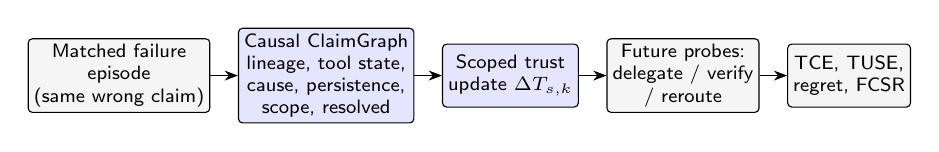
\begin{tikzpicture}[font=\sffamily\scriptsize, >=Stealth, node distance=3.5mm,
 box/.style={draw, rounded corners=1.5pt, minimum height=8mm, align=center, inner sep=2pt, fill=gray!8},
 hl/.style={box, fill=blue!10}]
 \node[box] (a) {Matched failure\\episode\\(same wrong claim)};
 \node[hl, right=of a] (b) {Causal ClaimGraph\\lineage, tool state,\\cause, persistence,\\scope, resolved};
 \node[hl, right=of b] (c) {Scoped trust\\update $\dT_{s,k}$};
 \node[box, right=of c] (d) {Future probes:\\delegate / verify\\/ reroute};
 \node[box, right=of d] (e) {TCE, TUSE,\\regret, FCSR};
 \draw[->] (a)--(b); \draw[->] (b)--(c); \draw[->] (c)--(d); \draw[->] (d)--(e);
\end{tikzpicture}}
\caption{Experimental flow. Only the cause varies across the four matched episodes. The graph's causal state is turned into a scoped trust update, which is scored against measured post-failure reliability.}
\label{fig:flow}
\end{figure}

\section{Method: Causal ClaimGraph}
\paragraph{Graph state.}
Every atomic claim is a node holding its claim id, parent claim, agent, skill, text, evidence, tool state, confidence and verification outcome. After diagnosis the node also records the failure cause, its persistence (transient, persistent or routing), its scope (which skill or skills it implicates) and whether it has been resolved. Keeping agent trust and claim trust apart is the point: a capable agent can emit a low-trust claim after a retrieval failure, and the graph lets the supervisor say so.


\begin{figure}[t]
\centering
\resizebox{\columnwidth}{!}{%
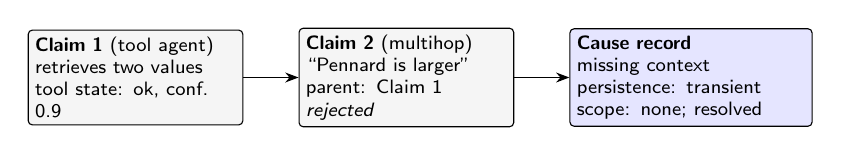
\begin{tikzpicture}[font=\sffamily\scriptsize, >=Stealth,
 n/.style={draw, rounded corners=1.5pt, align=left, inner sep=2.5pt, fill=gray!8, text width=2.55cm},
 c/.style={draw, rounded corners=1.5pt, align=left, inner sep=2.5pt, fill=blue!10, text width=2.9cm}]
 \node[n] (p) {\textbf{Claim 1} (tool agent)\\retrieves two values\\tool state: ok, conf.\ 0.9};
 \node[n, right=7mm of p] (q) {\textbf{Claim 2} (multihop)\\``Pennard is larger''\\parent: Claim 1\\\emph{rejected}};
 \node[c, right=7mm of q] (r) {\textbf{Cause record}\\missing context\\persistence: transient\\scope: none; resolved};
 \draw[->] (p)--(q); \draw[->] (q)--(r);
\end{tikzpicture}}
\caption{A schematic ClaimGraph fragment (invented values for illustration). The cause record is what the supervisor turns into a scoped trust update.}
\label{fig:graph}
\end{figure}

\paragraph{Memory conditions.}
The supervisor LLM receives one of the following states and returns $\dT_{s,k}$ for each skill and a cause attribution.
\emph{No memory} sees only the rejection.
\emph{Raw history} sees the original recommendation, the rejection and the subagent's transcript, with and without chain-of-thought.
\emph{Outcome-only} sees success or failure.
\emph{Skill-conditioned} attaches the failure to a skill.
\emph{ClaimGraph} sees the provenance together with cause, persistence, scope and resolution.
\emph{ClaimGraph, cause masked} sees the same graph without the explicit cause fields, so the cause must be inferred from evidence provided versus required and tool state.
Three rule-based conditions replace the LLM's magnitude with a fixed update given a cause: \emph{true cause} uses the oracle label, \emph{fit} uses rule values fit on non-test episodes, and \emph{inferred cause} first has the LLM infer the cause from the masked graph and then applies the rule.

\paragraph{Scoped update rule.}
Given a cause $c$, the rule sets
\begin{equation}
\dT_{s,k}=\begin{cases}
0 & c\in\{\mathrm{MC},\mathrm{TF}\}\\[2pt]
-0.10 & c=\mathrm{OOS},\ k=k_{\text{task}}\\[2pt]
-0.30\ /\ {-0.05} & c=\mathrm{PR},\ k=\text{same}\ /\ \text{near}\\[2pt]
0 & \text{all other skills,}
\end{cases}
\end{equation}
where MC is missing context, TF tool failure, OOS out-of-specialty, PR persistent reasoning, and $k_{\text{task}}$ is the skill the misrouted task needed.
The values are a hand-set prior, so this condition is best read as an upper bound on what cause-aware updating can deliver once the cause is known. The \emph{fit} variant refits the constants on non-test episodes and performs about the same.


\paragraph{Ablations.}
We remove, one at a time, the parent links, the tool state, and the persistence and resolution fields, and we mask the explicit cause fields.

\section{Experimental Setup}
\paragraph{Models.}
One supervisor and four specialists share a base model, with different prompts and tool permissions. We run GPT-4o-mini, Claude Haiku 5.5 and Llama-3.3-70B-Instruct, all through OpenRouter at temperature $0.7$ with $3$ seeds. A heterogeneous team uses a GPT-4o-mini supervisor with Haiku as the fact agent, Llama as the multi-hop agent and GPT-4o-mini for the quantitative and tool agents.

\paragraph{Statistics.}
Comparisons are paired at the base-task level. We report cluster-bootstrap confidence intervals, Wilcoxon signed-rank tests with Holm correction, exact McNemar tests on whether the supervisor delegates correctly on both same-skill probes, and a mixed-effects model with crossed variance components for base task and model family.

\paragraph{Implementation.}
Supervisor and specialist prompts are fixed across conditions apart from the memory block. The supervisor returns structured JSON, which we parse with a repair step for common malformations such as a missing closing bracket, falling back to extracting the scalar answer when needed. A reply that still cannot be parsed is scored as no cause and no trust change. All model calls go through a disk cache, which makes reruns of the same code cheap and repeatable.

\begin{table*}[t]
\centering\small
\begin{tabular}{lccccccc}
\toprule
Memory condition & TCE$\downarrow$ & TUSE$\downarrow$ & Regret$\downarrow$ & FCSR$\downarrow$ & Over-dist.$\downarrow$ & Under-dist.$\downarrow$ & Success$\uparrow$\\
\midrule
No memory & 0.064 & 0.025 & 0.068 & 0.159 & 0.098 & 0.267 & 0.825 \\
Raw history & 0.069 & 0.043 & 0.041 & 0.111 & 0.172 & 0.218 & 0.836 \\
Outcome-only & 0.068 & 0.032 & 0.050 & 0.126 & 0.208 & 0.271 & 0.836 \\
Skill-conditioned & 0.048 & \textbf{0.014} & 0.039 & 0.121 & 0.222 & 0.188 & 0.837 \\
ClaimGraph, cause masked & 0.055 & 0.022 & 0.040 & 0.117 & 0.235 & 0.186 & 0.838 \\
ClaimGraph & 0.054 & 0.018 & \textbf{0.029} & \textbf{0.104} & 0.182 & 0.123 & 0.839 \\
ClaimGraph + rule (inferred cause) & \textbf{0.043} & 0.019 & 0.030 & 0.115 & \textbf{0.116} & \textbf{0.076} & \textbf{0.840} \\
\midrule
ClaimGraph + rule (true cause) & 0.024 & 0.003 & 0.005 & 0.115 & 0.000 & 0.041 & 0.845 \\
\bottomrule
\end{tabular}
\caption{Test split, mean over three model families (GPT-4o-mini, Haiku 5.5, Llama-3.3-70B). Bold marks the best row among those that do not use the oracle cause. The true-cause rule is an upper bound, not a deployable condition. FCSR is not reduced by it (0.115 against 0.104 for the graph), so FCSR does not move monotonically with calibration.}
\label{tab:main}
\end{table*}

\section{Results}
\paragraph{Outcome-only memory miscalibrates in both directions (H1, H3).}
Figure~\ref{fig:signed} plots the signed error $\dT-\dTs$ on the affected skill. After resolved transient failures (missing context, tool failure) almost every condition over-penalizes, by roughly $0.10$ to $0.18$ against a target of zero; the exceptions are the no-memory baseline ($-0.06$) and the inferred-cause rule on tool failure ($-0.06$). Table~\ref{tab:signed} gives the numbers behind the figure. After persistent reasoning failures every condition under-reacts. Outcome-only memory sits $+0.24$ above the target, the graph $+0.14$, the inferred-cause rule $+0.08$ and the true-cause rule $+0.04$. For out-of-specialty failures outcome-only memory under-penalizes the misrouted skill ($+0.13$), whereas the graph overshoots in the other direction ($-0.09$). In short, a supervisor that sees only outcomes punishes the wrong agents for the wrong reasons and then does not punish the weak one enough.

\begin{figure}[t]
\centering
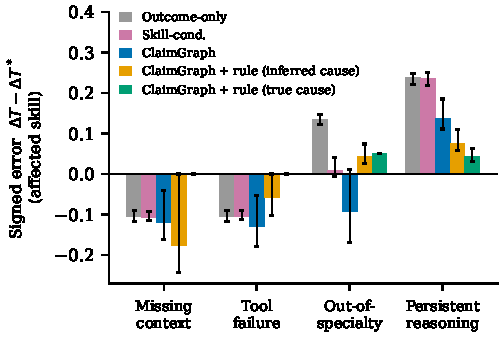
\includegraphics[width=\columnwidth]{figs/fig_signed.pdf}
\caption{Signed trust error on the affected skill by cause (mean over four runs; bars show min--max across runs). Zero is ideal. Negative means over-penalizing, positive means under-reacting.}
\label{fig:signed}
\end{figure}

\begin{table}[t]
\centering\scriptsize
\setlength{\tabcolsep}{3pt}
\begin{tabular}{lcccc}
\toprule
Condition & Missing ctx. & Tool fail. & Out-of-spec. & Persistent\\
\midrule
No memory & -0.058 & -0.058 & +0.117 & +0.284 \\
Raw history & -0.110 & -0.119 & +0.057 & +0.176 \\
Outcome-only & -0.104 & -0.104 & +0.134 & +0.238 \\
Skill-cond. & -0.107 & -0.106 & +0.009 & +0.236 \\
ClaimGraph & -0.119 & -0.130 & -0.094 & +0.138 \\
Graph+rule (inf.) & -0.177 & -0.057 & +0.044 & +0.076 \\
Graph+rule (true) & +0.000 & +0.000 & +0.050 & +0.043 \\
\bottomrule
\end{tabular}
\caption{Signed error $\dT-\dTs$ on the affected skill, mean over four runs. Negative means over-penalizing, positive means under-reacting.}
\label{tab:signed}
\end{table}

Table~\ref{tab:hyp} summarizes where each hypothesis stands. H2 deserves a note. Spillover is not a problem of outcome-only memory, which has no skill to spill from, but of transcript-based conditions: with raw history supervisors often spread a penalty onto skills that were not at fault.

\begin{table}[t]
\centering\scriptsize
\setlength{\tabcolsep}{3pt}
\begin{tabular}{p{0.9cm}p{2.1cm}p{4.2cm}}
\toprule
 & Verdict & Main evidence\\
\midrule
H1 & Supported & Over-penalty of roughly $0.10$--$0.18$ on missing context and tool failure under almost every condition (Table~\ref{tab:signed})\\
H2 & Partly supported & Spillover onto unaffected skills is common with raw history (174 cases), rare with outcome-only memory (40) and absent with skill memory (0)\\
H3 & Supported & Under-reaction of $+0.24$ for outcome-only and skill memory (Table~\ref{tab:signed})\\
H4 & Supported with the true cause; partial otherwise & TCE $0.024$ with the oracle rule; $0.043$ with inferred cause; graph alone mixed across models\\
\bottomrule
\end{tabular}
\caption{Verdicts on the four hypotheses.}
\label{tab:hyp}
\end{table}

\paragraph{The graph helps, and an explicit rule helps much more (H4).}
Table~\ref{tab:main} gives pooled results. Relative to outcome-only memory, the ClaimGraph lowers regret ($0.050\to0.029$), TUSE ($0.032\to0.018$), under-distrust ($0.271\to0.123$) and FCSR ($0.126\to0.104$). It also wins the exact McNemar test on correct same-skill delegation, with 383 episodes where only the graph is right against 67 where only outcome-only is ($p<10^{-50}$). The rule driven by the true cause is far stronger: TCE $0.024$, TUSE $0.003$, regret $0.005$, and 825 discordant episodes in its favor against none. That tells us the cause label carries the signal, and that an LLM handed the same label still does not map it onto the right magnitude. Replacing the oracle label with the LLM-inferred cause keeps part of the gain (TCE $0.043$, regret $0.030$, under-distrust $0.076$).

\begin{table}[t]
\centering\scriptsize
\setlength{\tabcolsep}{2.4pt}
\begin{tabular}{llccccc}
\toprule
Run & Condition & TCE & TUSE & Regret & Over & Under\\
\midrule
GPT-4o-mini & Outcome-only & 0.068 & 0.032 & 0.050 & 0.000 & 0.281 \\
 & Skill-cond. & 0.047 & 0.014 & 0.040 & 0.040 & 0.188 \\
 & ClaimGraph & 0.069 & 0.025 & 0.040 & 0.115 & 0.121 \\
 & Graph+rule (inf.) & 0.050 & 0.026 & 0.035 & 0.148 & 0.069 \\
 & Graph+rule (true) & 0.024 & 0.003 & 0.005 & 0.000 & 0.062 \\
\midrule
Haiku 5.5 & Outcome-only & 0.067 & 0.029 & 0.059 & 0.375 & 0.292 \\
 & Skill-cond. & 0.052 & 0.017 & 0.044 & 0.375 & 0.188 \\
 & ClaimGraph & 0.038 & 0.006 & 0.022 & 0.181 & 0.123 \\
 & Graph+rule (inf.) & 0.030 & 0.003 & 0.022 & 0.000 & 0.115 \\
 & Graph+rule (true) & 0.025 & 0.003 & 0.006 & 0.000 & 0.062 \\
\midrule
Llama-3.3-70B & Outcome-only & 0.068 & 0.036 & 0.042 & 0.250 & 0.240 \\
 & Skill-cond. & 0.045 & 0.011 & 0.032 & 0.250 & 0.188 \\
 & ClaimGraph & 0.055 & 0.022 & 0.026 & 0.250 & 0.125 \\
 & Graph+rule (inf.) & 0.049 & 0.028 & 0.032 & 0.200 & 0.044 \\
 & Graph+rule (true) & 0.022 & 0.003 & 0.003 & 0.000 & 0.000 \\
\midrule
Hetero team & Outcome-only & 0.066 & 0.026 & 0.043 & 0.125 & 0.281 \\
 & Skill-cond. & 0.048 & 0.014 & 0.032 & 0.125 & 0.188 \\
 & ClaimGraph & 0.075 & 0.021 & 0.031 & 0.133 & 0.138 \\
 & Graph+rule (inf.) & 0.047 & 0.021 & 0.028 & 0.187 & 0.023 \\
 & Graph+rule (true) & 0.024 & 0.000 & 0.003 & 0.000 & 0.000 \\
\bottomrule
\end{tabular}
\caption{Per-run results on the test split. Over/Under are over- and under-distrust rates on same-skill probes.}
\label{tab:runs}
\end{table}

\paragraph{The effect depends on the model (a negative result).}
Table~\ref{tab:runs} splits the pooled numbers by run, and Table~\ref{tab:contrast} gives paired differences. The graph's advantage over outcome-only memory on TCE holds for Haiku ($-0.029$) and Llama ($-0.013$), vanishes for GPT-4o-mini ($+0.001$), and reverses slightly for the heterogeneous team ($+0.009$). Against the skill-conditioned baseline the picture is less flattering still. Skill conditioning already localizes the penalty (pooled TUSE $0.014$, the best of any LLM condition), while the graph spreads some penalty onto unaffected skills, so the graph has higher TCE than skill memory in three of four runs. Its regret advantage over skill memory is small and significant only for Haiku and Llama. Only Haiku satisfies the full check that the graph beats both baselines on TCE and regret, and we do not claim a general superiority of the graph over skill-conditioned memory.

\begin{table}[t]
\centering\scriptsize
\setlength{\tabcolsep}{2.6pt}
\begin{tabular}{lccccccc}
\toprule
 & \multicolumn{3}{c}{Graph $-$ Outcome} & \multicolumn{2}{c}{Graph $-$ Skill} & \multicolumn{2}{c}{Rule(inf.) $-$ Outc.}\\
\cmidrule(lr){2-4}\cmidrule(lr){5-6}\cmidrule(lr){7-8}
Run & TCE & TUSE & Reg. & TCE & Reg. & TCE & Reg.\\
\midrule
GPT-4o-mini & +0.001 & -0.007$^{*}$ & -0.010$^{*}$ & +0.022$^{*}$ & +0.000 & -0.019$^{*}$ & -0.015 \\
Haiku 5.5 & -0.029$^{*}$ & -0.023$^{*}$ & -0.037$^{*}$ & -0.014$^{*}$ & -0.022$^{*}$ & -0.038$^{*}$ & -0.037$^{*}$ \\
Llama-3.3-70B & -0.013$^{*}$ & -0.014$^{*}$ & -0.016$^{*}$ & +0.010$^{*}$ & -0.005$^{*}$ & -0.018$^{*}$ & -0.010 \\
Hetero team & +0.009$^{*}$ & -0.005$^{*}$ & -0.012$^{*}$ & +0.027$^{*}$ & -0.001 & -0.019$^{*}$ & -0.015$^{*}$ \\
\bottomrule
\end{tabular}
\caption{Paired differences (negative favors the first condition). $^{*}$: Holm-corrected Wilcoxon $p<0.05$ over base-task means.}
\label{tab:contrast}
\end{table}

\paragraph{Where the regret reduction comes from.}
Table~\ref{tab:cause} breaks regret down by cause. For missing context and tool failure, where the right action is to keep delegating, no memory condition is much worse than any other (regret $0.01$ to $0.03$), and the graph is not worse than outcome-only memory. The gains concentrate where the future really changed. For out-of-specialty failures the graph and skill memory remove the regret that outcome-only memory carries ($0.040\to0.000$), and for persistent weakness regret falls from $0.103$ to $0.069$, against $0.016$ for the true-cause rule. The mixed-effects model on the three single-model runs (Table~\ref{tab:mixed}) agrees: the graph's regret reduction is concentrated in out-of-specialty failures (interaction $-0.029$, 95\% CI $[-0.043,-0.015]$) and persistent failures ($-0.018$, $[-0.031,-0.004]$), with only a small effect on missing context ($-0.012$). The inferred-cause rule shows the cost of mislabeling: its regret on missing context ($0.054$) is the highest of any condition, because a misread cause turns a target of zero into a persistent penalty.

\begin{table}[t]
\centering\scriptsize
\setlength{\tabcolsep}{3pt}
\begin{tabular}{lcccc}
\toprule
Condition & Missing ctx. & Tool fail. & Out-of-spec. & Persistent\\
\midrule
No memory & 0.010 & 0.011 & 0.029 & 0.212 \\
Raw history & 0.022 & 0.025 & 0.021 & 0.095 \\
Outcome-only & 0.026 & 0.026 & 0.040 & 0.103 \\
Skill-cond. & 0.027 & 0.027 & 0.000 & 0.093 \\
ClaimGraph & 0.022 & 0.029 & 0.000 & 0.069 \\
Graph+rule (inf.) & 0.054 & 0.010 & 0.002 & 0.051 \\
Graph+rule (true) & 0.000 & 0.000 & 0.000 & 0.016 \\
\bottomrule
\end{tabular}
\caption{Delegation regret by true cause, mean over four runs.}
\label{tab:cause}
\end{table}


\begin{table*}[t]
\centering\small
\begin{tabular}{llccc}
\toprule
Condition (vs.\ outcome-only) & Metric & At missing context & $\times$ out-of-specialty & $\times$ persistent\\
\midrule
ClaimGraph & TCE & $-0.010$ [-0.016, -0.005] & $-0.034$ [-0.042, -0.026] & $+0.013$ [+0.005, +0.021] \\
 & Regret & $-0.012$ [-0.022, -0.002] & $-0.029$ [-0.043, -0.015] & $-0.018$ [-0.031, -0.004] \\
\midrule
Skill-cond. & TCE & $-0.009$ [-0.015, -0.003] & $-0.047$ [-0.055, -0.040] & $+0.008$ [+0.000, +0.016] \\
 & Regret & $+0.000$ [-0.009, +0.010] & $-0.041$ [-0.055, -0.027] & $-0.008$ [-0.022, +0.006] \\
\midrule
Graph+rule (true) & TCE & $-0.037$ [-0.042, -0.031] & $-0.019$ [-0.027, -0.011] & $-0.008$ [-0.016, -0.001] \\
 & Regret & $-0.030$ [-0.040, -0.020] & $-0.010$ [-0.024, +0.003] & $-0.048$ [-0.062, -0.034] \\
\bottomrule
\end{tabular}
\caption{Mixed-effects estimates (3 families, crossed variance components for base task and model family). The first column is the effect at the reference cause, missing context; the other two are interaction terms added to it. Entries are coefficients with 95\% confidence intervals. For transient causes the target is zero, so TCE and TUSE coincide there.}
\label{tab:mixed}
\end{table*}

\paragraph{Skill memory is a strong baseline.}
The same model shows how competitive skill-conditioned memory is. On out-of-specialty failures it reduces both TCE ($-0.047$) and regret ($-0.041$) by more than the graph does ($-0.034$ and $-0.029$), because attaching the failure to the skill is exactly the information a routing error calls for. The graph earns its keep on persistent weakness, where its regret reduction ($-0.018$) is larger than skill memory's ($-0.008$, interval including zero), and the rule driven by the true cause is better still ($-0.048$). Put differently, the skill label buys scope and the cause buys magnitude.

\paragraph{How the supervisor behaves.}
Table~\ref{tab:beh} shows the actions behind these numbers. Outcome-only memory verifies most often ($0.53$) and reroutes least ($0.44$), and wastes the most verification effort on claims that were actually fine ($0.245$ redundant verifications). The graph and especially the rules shift effort from verification to rerouting and cut redundant verification to $0.13$ and $0.03$--$0.06$. Mean utility rises only from $0.835$ to $0.846$ even with the true cause, probably because the utilities of the three actions are close on many probes, which is one reason we report decisions as well as utility.

\begin{table}[t]
\centering\scriptsize
\setlength{\tabcolsep}{3pt}
\begin{tabular}{lcccc}
\toprule
Condition & Verify & Reroute & Redund.\ verify & Utility\\
\midrule
No memory & 0.439 & 0.442 & 0.149 & 0.831 \\
Raw history & 0.436 & 0.513 & 0.185 & 0.837 \\
Outcome-only & 0.534 & 0.439 & 0.245 & 0.835 \\
Skill-cond. & 0.516 & 0.444 & 0.194 & 0.838 \\
ClaimGraph & 0.419 & 0.526 & 0.129 & 0.840 \\
Graph+rule (inf.) & 0.343 & 0.555 & 0.058 & 0.840 \\
Graph+rule (true) & 0.367 & 0.514 & 0.034 & 0.846 \\
\bottomrule
\end{tabular}
\caption{Supervisor behavior on future probes, mean over four runs. Redundant verification is verification of a claim that was correct.}
\label{tab:beh}
\end{table}

\paragraph{Ablations.}
Table~\ref{tab:abl} reports each ablation minus the full graph, averaged over four runs, with in parentheses the number of runs whose confidence interval excludes zero. Parent links make almost no difference, which tells us that in these short episodes the lineage is not what the supervisor uses, even though the extractor recovers it reliably. Removing the persistence and resolution fields hurts TUSE and FCSR in all four runs (TUSE $+0.005$, FCSR $+0.013$), so these fields carry real information about scope and about whether a claim should survive. Removing tool state has little effect on TCE or FCSR and a small, inconsistent effect on scope and regret. Masking the cause fields raises regret, TUSE and FCSR in three of four runs; the mean TCE change is within noise. Two of the ablations (persistence, cause fields) slightly \emph{lower} TCE in some runs while raising regret and scope error, a reminder that TCE alone is not enough.

\begin{table}[t]
\centering\scriptsize
\setlength{\tabcolsep}{2.5pt}
\begin{tabular}{lcccc}
\toprule
Ablation & TCE & TUSE & Regret & FCSR\\
\midrule
Remove cause fields (masked) & $-0.003$ (3) & $+0.005$ (3) & $+0.009$ (3) & $+0.014$ (3) \\
Remove parent links & $+0.001$ (0) & $+0.000$ (0) & $-0.000$ (0) & $+0.001$ (1) \\
Remove tool state & $+0.001$ (1) & $+0.002$ (4) & $+0.002$ (2) & $-0.002$ (1) \\
Remove persistence/resolution & $-0.003$ (4) & $+0.005$ (4) & $+0.004$ (2) & $+0.013$ (4) \\
\bottomrule
\end{tabular}
\caption{Ablation minus full graph (positive means the ablation is worse), mean over four runs; in parentheses, the number of runs whose 95\% CI excludes zero.}
\label{tab:abl}
\end{table}

\begin{figure}[t]
\centering
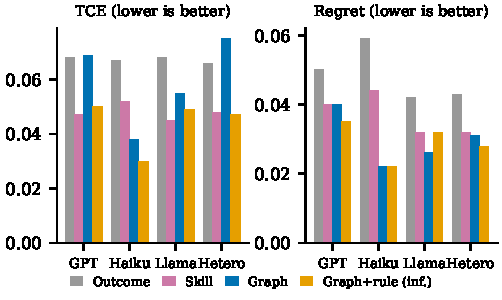
\includegraphics[width=\columnwidth]{figs/fig_models.pdf}
\caption{TCE and regret per run. The graph helps most on Haiku. On GPT-4o-mini and the heterogeneous team it does not reduce TCE relative to outcome-only memory.}
\label{fig:models}
\end{figure}

\paragraph{Why the inferred-cause rule falls short.}

Attribution accuracy rises from $0.25$ for outcome-only and $0.46$ for skill memory to $0.76$ for raw history and $0.71$ for the masked graph. With explicit cause fields it is $1.00$ by construction, which only shows that the label gets read. From the masked graph the model identifies tool failure ($0.72$), out-of-specialty ($0.94$) and persistent reasoning ($0.89$) well, but gets missing context right only $28\%$ of the time, compared with $83\%$ from raw history. It does not make use of the fields recording items provided versus items required. That misattribution (647 of 1{,}920 episode-condition pairs, for both the masked and inferred-rule conditions) is what makes the inferred rule over-penalize missing context most ($-0.18$ in Figure~\ref{fig:signed}). The provenance extractor itself is dependable: origin agent $0.97$ to $1.00$, lineage $0.97$ to $1.00$, tool dependency $0.86$ to $0.97$ and joint origin--source--tool $0.79$ to $0.88$ across runs.


\begin{table}[t]
\centering\scriptsize
\setlength{\tabcolsep}{3pt}
\begin{tabular}{lccccc}
\toprule
Condition & Overall & Missing ctx. & Tool fail. & Out-of-spec. & Persistent\\
\midrule
No memory & 0.25 & 0.15 & 0.03 & 0.71 & 0.11 \\
Raw history & 0.76 & 0.83 & 0.60 & 0.65 & 0.97 \\
Raw + CoT & 0.76 & 0.85 & 0.58 & 0.61 & 0.95 \\
Outcome-only & 0.25 & 0.08 & 0.11 & 0.66 & 0.15 \\
Skill-cond. & 0.46 & 0.06 & 0.25 & 1.00 & 0.54 \\
Graph, masked & 0.71 & 0.28 & 0.72 & 0.94 & 0.89 \\
ClaimGraph & 1.00 & 1.00 & 1.00 & 1.00 & 1.00 \\
\bottomrule
\end{tabular}
\caption{Cause-attribution accuracy by true cause, mean over four runs. The explicit graph carries the label, so its $1.00$ is by construction.}
\label{tab:attr}
\end{table}

Table~\ref{tab:attr} shows how differently the conditions fail. Raw history is strong on missing context and persistent reasoning but poor on tool failure ($0.60$) and out-of-specialty ($0.65$), where the subagent's own account is least reliable. Outcome-only memory sits at chance for four classes ($0.25$), since it has little to go on, and skill memory does only somewhat better. The masked graph is the opposite: it recovers routing errors well ($0.94$) and misses missing context. The conditions are therefore complementary, which suggests combining the transcript with the graph's evidence fields for cause inference.

\paragraph{Provenance quality.}
In the GPT-4o-mini run, joint origin--source--tool accuracy is lowest on GSM8K (0.81) and on out-of-specialty episodes (0.78), and perfect on the synthetic tool tasks, where evidence is a clean table. Provenance errors therefore concentrate on tasks whose evidence is free text or arithmetic, not on the cause itself.

\paragraph{Heterogeneous team.}
Mixing models does not rescue the graph. With a GPT-4o-mini supervisor the team's graph TCE is $0.075$ against $0.066$ for outcome-only memory, while regret improves ($0.043\to0.031$) and FCSR improves ($0.148\to0.116$). This is consistent with the supervisor's own tendency to spread penalties mattering more than the specialists beneath it, and it matches the GPT-4o-mini single-model run, but we did not isolate this with a separate experiment.

\paragraph{Cost and benefit.}
Real downstream success on the future probes is nearly identical across conditions ($0.825$ to $0.845$), so the benefit is in oversight decisions rather than task accuracy. Graph prompts are about $2.8\times$ longer than outcome-only prompts ($894$ against $320$ tokens on average), while completion length is about the same ($149$ against $158$ tokens). The explicit rule adds no inference cost beyond cause identification.

\section{Case Study: How Subagent and Supervisor Misalign}
Numbers say that supervisors err; they do not say how. We classified each episode-condition pair (1{,}920 per condition over four runs) with a fixed rule-based taxonomy, and Table~\ref{tab:tax} gives the counts. The examples that follow come from the automatically generated case-study files, which list episodes by TCE within each category. We picked the ones that illustrate each type, and the run and condition are given for each. They are illustrations, not a representative sample.

\begin{table}[t]
\centering\scriptsize
\setlength{\tabcolsep}{3pt}
\begin{tabular}{lcccccc}
\toprule
Misalignment type & Raw & Outc. & Skill & Mask. & Graph & G+rule\\
\midrule
Blamed for context & 177 & 81 & 81 & 275 & 204 & 254 \\
Blamed for tool fault & 215 & 82 & 78 & 284 & 230 & 83 \\
Cause misattributed & 269 & 1442 & 1030 & 647 & 1 & 647 \\
Misled by self-report & 231 & 0 & 0 & 0 & 0 & 0 \\
Routing$\to$specialty penalized & 152 & 82 & 0 & 68 & 28 & 0 \\
Scope spillover & 174 & 40 & 0 & 13 & 14 & 0 \\
Persistent under-reaction & 339 & 390 & 390 & 355 & 283 & 196 \\
\bottomrule
\end{tabular}
\caption{Counts of misalignment types over four runs (multi-label; G+rule uses the inferred cause).}
\label{tab:tax}
\end{table}

\paragraph{The subagent's own account misleads the lead.}
A subagent's self-report is part of the raw transcript, and in 231 raw-history decisions the supervisor followed a self-report that named the wrong cause. In \texttt{tool\_synth-40} (Haiku, raw history; true cause out-of-specialty, multi-hop agent) the subagent said ``I had all the information I needed; my reasoning was wrong.'' The supervisor concluded persistent reasoning and cut multi-hop trust by $0.25$, while the oracle penalizes only the tool skill ($-0.15$). The same self-report appears in \texttt{tool\_synth-25} (Haiku, raw with chain-of-thought), where the supervisor cut the fact agent's trust by $0.25$ instead. In \texttt{hotpotqa-35} (GPT-4o-mini, raw with chain-of-thought; true cause missing context) the self-report blamed an unreliable retrieval tool, the supervisor adopted ``tool failure'' and cut fact and multi-hop trust by $0.50$ each against a target of zero. This category is zero for conditions without the transcript and for the graph, whose cause field does not come from the self-report.

\paragraph{Blaming the agent for context or tool faults.}
The graph does not remove this failure. Blame for context faults is 204 in the graph condition against 81 for outcome-only memory, and for tool faults 230 against 82. Outcome-only supervisors look better only because they rarely commit to a cause at all (1{,}442 cause misattributions); graph supervisors name the cause, often correctly, and still lower trust.

\paragraph{Right cause, wrong magnitude.}
In \texttt{tool\_synth-38} (GPT-4o-mini, graph with parent links removed) the supervisor attributed the failure correctly to missing context and then cut fact, multi-hop and quantitative trust by $0.20$ each and tool trust by $0.30$, with a rationale that the agent ``failed to provide sufficient evidence''. The target was zero on every skill and the regret was $0.16$. In \texttt{gsm8k-51} (GPT-4o-mini, graph) it again attributed missing context correctly yet cut quantitative trust by $0.20$. Correct attribution is necessary but not sufficient, which is exactly why the explicit rule helps.

\paragraph{Penalizing the true specialty.}
In \texttt{hotpotqa-8} (Haiku, outcome-only; true cause out-of-specialty, tool agent) the supervisor reasoned that the failure fell within the tool agent's declared specialty, whose prior reliability was $1.00$, and cut tool trust by $0.30$. The oracle penalty was $-0.15$ on the multi-hop skill, the skill the task actually needed. This pattern of penalizing the agent's own specialty for a routing error appears 152 times with raw history and 82 times with outcome-only memory, against 28 with the graph and none with skill memory.

\paragraph{A benchmark artifact.}
Because the final wrong claim is scripted, some raw transcripts show retrieved evidence that contradicts the final answer, and supervisors reasonably read that as a reasoning failure. In \texttt{tool\_synth-23} (Haiku, raw history) a tool failure was attributed to persistent reasoning and tool trust was cut by $0.40$. The retrieved rows showed the right answer, the agent's own steps agreed, and the final answer contradicted both. This inflates raw-history error on tool-failure cases and is a limitation of forced-claim construction.

\section{Discussion and Limitations}
\paragraph{What the results mean.}
The consistent finding is that the cause, once known, is worth a lot, and that obtaining and using it is the hard part. The graph gives the supervisor useful structure, but the supervisor still converts that structure into trust changes unevenly across models. A skill-conditioned baseline captures much of the scope benefit cheaply. The practical reading is that causal state is most valuable when paired with an explicit update rule, and when cause inference is reliable enough to drive it.

\paragraph{Guidance for builders.}
Three practical points follow from the evidence. If cost matters most, attach failures to skills: skill-conditioned memory is nearly as cheap as outcome-only memory and removes most routing regret. If persistent weaknesses matter, record the cause and its persistence, because those fields are what separate a weak agent from a failed tool. And if the cause can be established reliably, for example because the tool layer reports its own errors, apply an explicit scoped rule rather than asking the model to size the penalty; in our runs the rule with the true cause cut regret by about a factor of six relative to the graph alone ($0.029\to0.005$).

\paragraph{Relation to existing reputation systems.}
Our skill-conditioned baseline stands in for context-aware reputation designs \citep{xia2026conditional,chishti2026agentreputation}. We did not re-implement those systems, only the idea of attaching trust to a skill, so the comparison says how far skill scoping goes when the update is otherwise outcome-driven and does not evaluate those systems themselves.

\paragraph{Scope and scale.}
The test split has 40 base tasks per run, one temperature, and three model families through one API provider; the tool tasks are synthetic.

\paragraph{Controlled profiles.}
Persistent weakness is induced by seeded answer corruption, so effect sizes depend on the corruption rates and on the utility parameters. The true-cause rule uses ground-truth labels and a hand-set table, so it bounds what cause-aware updating can achieve and does not demonstrate a deployable system.

\paragraph{Post-hoc choices.}
After inspecting an initial GPT-4o-mini run we (i) redefined over- and under-distrust relative to the oracle action, (ii) set the out-of-specialty routing penalty to $0.15$ as in the design, (iii) stratified the split by source, and (iv) repaired malformed JSON replies from Llama (a first Llama run was largely unusable because of unparseable output), which also changed GPT-4o-mini's calibrated profiles. Roughly 5 to 9\% of replies remain unparseable. All reported runs use the final code. The mixed-effects model covers the three single-model runs, and the heterogeneous team is analyzed separately.

\paragraph{Cost.} Graph prompts are $2.8\times$ longer than outcome-only prompts, and latency differences across providers make wall-clock comparisons unreliable.

\section{Future Directions}
Three directions follow from the negative results. First, cause inference should use both the transcript and the graph's evidence fields, since Table~\ref{tab:attr} shows their strengths are complementary: raw history reads persistent weakness and missing context well, while the masked graph reads routing. Second, the update rule should be learned or calibrated online rather than set by hand, and its constants checked against drift in an agent's true reliability. Third, the benchmark should be extended with naturally occurring persistent weaknesses instead of seeded corruption, and with longer episodes in which failures of several causes accumulate.

\section{Ethics and Reproducibility}
The benchmark uses public datasets and synthetic tool tasks and involves no personal data. A system that lowers its trust in a subagent changes which components get work, so a miscalibrated update can quietly exclude a capable component or keep a weak one. This is the failure we measure, and we recommend keeping a human-readable cause record for every trust change. Episodes, interventions and splits are generated by seeded code, and all model calls go through a disk cache.

\section{Conclusion}
The same observable failure should not produce the same trust update. In a matched counterfactual benchmark, supervisors that see only outcomes over-penalize resolved transient failures and under-react to persistent ones. Giving them an explicit causal state improves regret and scope but not TCE uniformly, and an explicit scoped rule driven by the true cause nearly closes the gap. The open problem is reliable cause inference, especially recognizing missing context, so that the rule can run without oracle labels. Promising next steps are inferring the cause from the transcript and the graph's evidence fields together, since their strengths are complementary, and learning the update rule online instead of setting it by hand. We plan to release task identifiers, intervention templates, prompts, calibration profiles, evaluation code and seeds with the camera-ready version, where licensing permits.

\clearpage
\bibliography{refs}
\end{document}
